\chapter{Background} \label{background}
Synchronous DRAM (SDRAM) was first standardised by JEDEC in 1993, and is still the foundation for modern DDR3 and DDR4 memories \cite{standard2008double}. Although the memory architecture has been improved over the years, the fundamental design has mostly been left untouched. However, there are several emerging memory technologies which aim at creating an entirely new and improved designs, both at the very physical and functional level, as well as refined architecures.
\bigskip

While DRAM cells have been used for some time now in the industry, they still have their inherent problems with volatilty. There have been a number of attempts to decrease the dependence of DDR DRAM and introduce a type of Non-Volatile RAM (NVRAM). This could both replace the need for a secondary storage system or be used in place of DRAM, in order to thus reduce complexity, energy usage and cost. Since DRAM energy usage equal to more than 20\% of a system's total energy, finding a substitute without sacrificing performance has been a hot research topic\cite{4658649}. Solid State Drives (SSDs) have been available for quite some time, but the underlying technology -- NAND flash memory -- is limited, e.g., by its access time being several orders of magnitude slower than DRAM and that NAND cells ability to hold data deteriorates with each write. A multitude of alternative Non-Volatile Memories (NVM) have been presented; two with a lot of potential and research support being: Phase Change Memory (PCM) and Spin-Transfer Torque RAM (STT-RAM). The former has higher density, i.e. effectively decreasing cost per byte, but is about 2-4 and 10-100 times slower when reading and writing, respectively \cite{Qureshi:2009:SHP:1555754.1555760, 5388621}. In addition, PCM on its own uses more power and the storage cells degrade for every write operation, which lowers their expected lifetime.  Meanwhile, STT-RAM matches DRAM in density and read performance (access time and energy use) but is outperformed when writing \cite{6557176, 6027811}. STT-RAM also needs to be designed with a trade-off between read and write performance \cite{Wang_2013, Khvalkovskiy_2013}.
\bigskip

The shortcomings of PCM and STT-RAM can to some extent be overcome by adapting memory systems to their respective strong properties. PCM is situated to replace DRAM as main memory because of its potential of lower cost and increased density, while STT-RAM mostly is investigated to be used instead of SRAM in system caches because of its speed and endurance. However, neither technology is truly ready to replace current product lines. Because of the higher costs involved with both the manufacturing and integration as well as the development time needed to fully utilise their respective good properties, there is still some time until they will reach market. One exception, however, is Intel who has launched 3D-Xpoint as a commercial NVRAM alternative (branded Optane), which, according to the hardware community, is based on PCM \cite{jeongdong_2017}. This means that for the foreseeable future, variants of DRAM is going to continue to dominate the market. As such, the focus of this background is to describe how current memory technology can be adapted to accomodate for higher performance.
\bigskip

In this chapter, we will start by describing how circuits can be put in stacks and how memories can be put in similar configurations. Next is a high-level walk-through of how today's memories operate, and lastly we go on to explain how a few emerging, stacked memory technologies are designed and how they compare. 

\section{3D stacking}
The idea of stacking current chips on top of one another has been around for some time \cite{lee2000three, jacob2005predicting, black2006stacking}, but it has until recently not been technically possible to viably manufacture such devices; one of the big hurdles has been the thermal issues stacking entails \cite{5074080}. Stacking memory chips has grown in popularity as one possible solution to today's memory limitations. In theory, stacking can enable a larger amount of memory and computation units being fitted onto the same area, while also allowing higher bandwidths and increased energy efficiency\cite{Lee:2016:SMA:2836331.2832911}. Being designed to be integrated close to the processor, there will be shorter data paths to traverse when memory is accessed, which in turn means less energy spent on large off-chip buses and shorter communication time between processor and memory. However, having memories in three dimensions requires more global bitlines and global sense amplifiers, which, without care, will greatly increase the memory's power usage.
\bigskip

There are several ways to build and integrate stacked memories, 3D IC stacking or 2.5D stacking \cite{6248905, 5702702, 6248842}. Marinissen et al also detail a work-in-progress IEEE standard which additionally defines 5.5D stacking \cite{7519330}. These systems are generally referred to as System in Package (SiP). 2.5D stacking means that chips are put on top of a (passive) silicon interposer, as can be seen in figure \ref{2D-chip}. The connections which are used both within the interposer to connect the chips and between the stacked chips are denoted as Through Silicon Via (TSV) \cite{Lau2018, lau2012through}. Between each die there are also micro-bumps (<25 µm) to create the bond between them. While 3D IC integration also leverages TSV and micro-bumps, it provides a much smaller footprint as well as an (theoretical) order of magnitude higher efficiency, e.g., in terms of link power bandwidth per mm$^{2}$ \cite{6248968}. In addition, it is possible to manufacture stacked chips without micro-bumps and instead only rely on TSV, known as 3D Silicon Integration. The most widely accepted way of doing 3D Si integration is by stacking wafers on top of one another, with the drawback that good dies easily are stacked with bad dies, resulting in a non-functioning chip, i.e., the yields are very low. 3D Si integration has even better potential than 3D IC integration, and there are some proposed methods to alleviate this issue. One being wafer matching, where tested wafers are matched together based on the number of known good dies that would be put together, and another where individual good dies are placed on top of the wafer \cite{Taouil:2010:TCA:1931472.1931973}. There is as always the trade-off between manufacturability and cost, where sufficient and thorough testing can help predict which method is most suitable.

\begin{figure}[!ht]
\centering
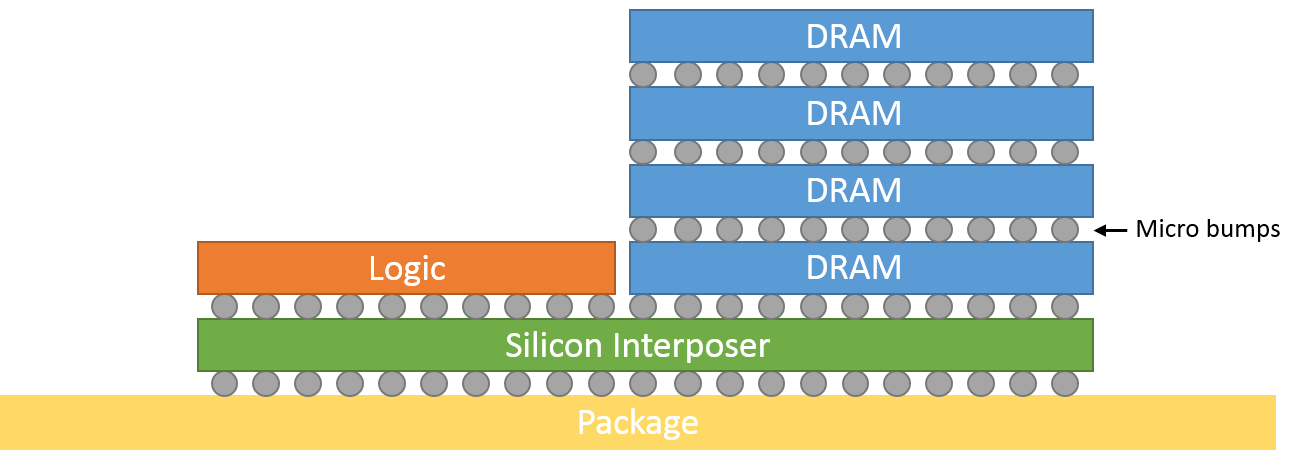
\includegraphics[width=0.75\linewidth]{figure/2D-integration.png}
\caption{Illustration of a 2.5D chip. The interposer is needed to enable communications between the Logic and DRAM. }
\label{2D-chip}
\end{figure}

\begin{figure}[!ht]
\centering
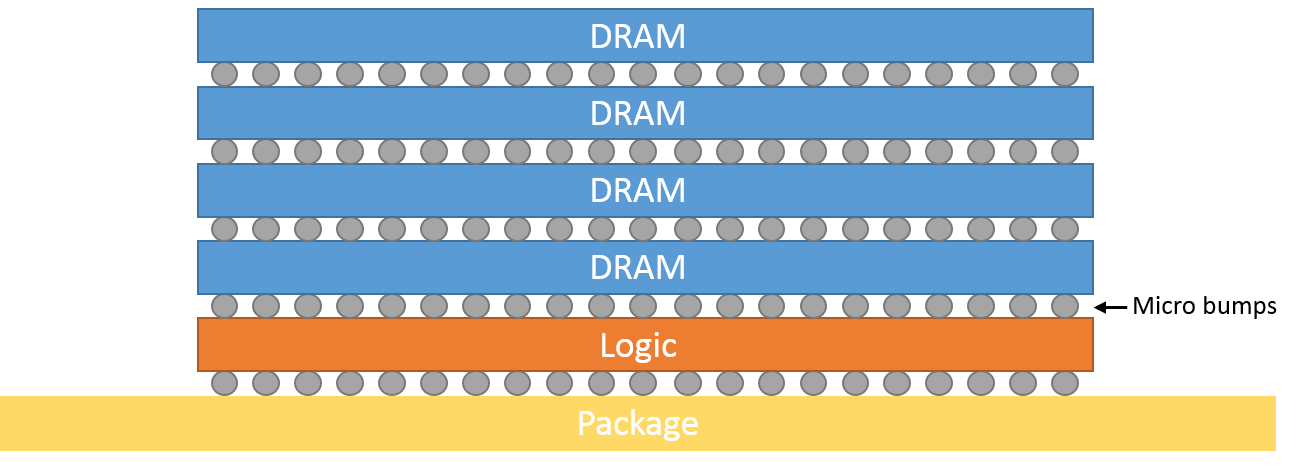
\includegraphics[width=0.75\linewidth]{figure/3D-integration.png}
\caption{Illustration of a 3D chip. All dies are directly connected through TSV.}
\label{3D-chip}
\end{figure}

Apart from introducing great potential in the future there are also some additional problems with stacking chips, e.g. verification and diverting thermal energy. There are several proposed methods of testing, where the underlying architecture could support both pre-bonding, mid-bonding and post-bonding tests. Pre-bonding tests are performed before and/or after doing wafer thinning, before dies are being stacked. When stacking, tests can be done on partial stacks, called mid-bond test, and complete stacks, called post-bond test. Enabling testing after initial bonding could include creating additional test pins to form a Test Access Port \cite{Marinissen:2012:CES:2492708.2493023}. Alternatively creating special probe pads, due to the difficulties in probing micro-bumps without risking damaging them \cite{5751450}. Furthermore, high performance chips will inevitably lead to heat generation and by putting them  on top of one another the heat cannot easily dissipate; since the space between the dies are too small for air or liquid to pass efficiently, there need to be some other thermal cooling mechanism \cite{5501261}. The optimal thermal scenario is when the hottest chip is placed on top, nearest a heat spreader, which is inherently true when doing 2.5D integration. Having 3D chips makes it more complicated, but separating the most heat generating dies as much as possible minimises in-package thermal transfer. This is one of several issues that has made 2.5D more realisable today, and still keeps 3D IC integration as a future goal. Due to the many advantages, performance-wise, with 3D stacking, it is very desirable to find a solution to this. Lastly, 3D stacking, compared to 2.5D, is also cheaper to manufacture because the package is smaller and less complex \cite{6263032}. This cost gap could, however, be lowered if the interposer die were to be tested before stacking, which could lead to an increased yield \cite{6542130}.


%%%%%%%%%%%%%%% STACKING MEMORIES %%%%%%%%%%%%%%%
\section{Stacking memories}
While stacking processing units is possible, they are often also the component generating the most heat in a system, and some benefits could be gained from stacking memory chips only. Having a stacked memory will by itself enable it to be denser and allow for more memory on the same die area. In addition, by having memory in multiple layers, it is also possible to place a separate memory controller in the memory stack. This gives the memory controller very close access to its resources and could allow for finer grained control over accesses and atomic memory operations ensured by the memory controller. This could off-load the CPU memory controller -- if one is needed at all!
\bigskip

There are a few noteworthy types of stacked memories: Hybrid Memory Cube (HMC), designed by Micron; High Bandwidth Memory (HBM), a JEDEC standard since 2013; and Wide-IO (WIO), also a JEDEC standard since 2011. While the two former are designed for 2.5D integration -- memory on the same substrate as the processor -- the latter supports 2.5D, but is primarily aimed for 3D integration. These three memory technologies are all based on conventional DRAM chips being stacked, but it could also be possible to stack other, emerging technologies as well. Wu et al. simulated full systems with today's SRAM cache setup and compared that to stacks of PCM and STT-RAM where the architecture took advantage of respective type's strengths, and their results showed notable IPC increases and energy use reduction with this setup \cite{Wu:2009:HCA:1555754.1555761}. More close at hand are the stacked memory cells in SSDs being produced, where the densest flash drives currently use 96 layers of NAND cells, commonly referred to as Vertical NAND (V-NAND) or 3D NAND \cite{tallis_2017}.
\bigskip

These memory technologies are all quite similar, but they primarily target different market segments. HMC is designed for high bandwidth at relatively high energy consumption and is comparatively expensive. This makes it more suitable for High Performance Computing (HPC) systems. HBM was designed specifically for graphics applications, and there have been multiple commercial products (graphics cards) utilising this memory type in recent years. Similarly to HMC, this technology is made for systems where adequate cooling is available and where a higher cost can be somewhat overlooked. WIO is, as opposed to the others, architectured for being integrated on top of System on Chips (SoCs). These types of systems are generally found in mobile devices, which is also what WIO is designed for. Like HBM, WIO hopes to increase the performance of the graphics processors, but inside mobile devices. These specific memory types are talked about in more detail in chapter \ref{background}.
\bigskip

Having memory far away running at high speeds will incur a great cost to power usage, and as such the most preferred way is to have memory as close to the processing unit as possible, but there is a BoM and manufacturing cost of having an interposer. However, many high performance x86 designs today use "chiplet" or Package-on-Package (PoP) designs, where modules, or clusters, of cores and caches are mounted onto an interposer and communicating over a high speed, extensible bus interface. By using this approach, some of the added cost of a larger interposer is already accounted for and should make it a little less costly to integrate stacked memories. There is, however, still no coming around the fact the tried and tested method of using DRAM DIMMs is still cheaper, but with the right workload the added performance could be worth the cost.
\bigskip

The tantalising option of increased bandwidth and potentially lower latency of stacked memories still has downsides apart from cost. Having stacked memory chips will close in the thermal energy generated and there is no way to easily dissipate it. Furthermore, (especially) stacked memories exhibit a positive feedback loop with respect to power usage, temperature and leakage power. When temperature rises, the DRAM leakage power will increase as well which will increase overall power consumption. A higher power consumption will create even more heat, and it might soon get out of hand \cite{4212027}. There are however suggested ways to mitigate this to some extent by making sure that allocations and accesses are spread out as much as possible inside the cube, thus taking the cube temperature into consideration when placing data and creating heat zones \cite{7252085}.
\bigskip

While these emerging types of memories are of interest on their own, whether they are non-volatile or standard DRAM, they could also be used in a Multi-Level Memory (MLM) design. An MLM design could utilise both the higher bandwidth of, e.g., HMC with the lower cost of DDR memory. A method has been described by Jayaraj et al \cite{Jayaraj:2015:PPM:2818950.2818976}, where HMC is being used as a scratchpad type memory while DDR is still being used as main memory. This results in a higher performance while at a lower Bill of Materials (BoM) cost compared to a system using only DDR. However, the added cost of designing such a system is not included and not all applications are memory bound enough to benefit. Furthermore, it would also be necessary for software developers to optimise their applications for this setup in order to see any major gains \cite{Bender:2015:KCT:2818950.2818977, BENDER2017213}. Lastly, it could be possible to use a hybrid-type memory using PCM memory with a DRAM buffer to hide or minimise the shortcomings of PCM, i.e. decrease latencies and write energy consumption \cite{Lee:2009:APC:1555815.1555758}.
\bigskip

In the end, NVRAM type of memories still belong to the future and stacked memories are the most realistic next step to take. Among the competing emerging DRAM technologies, HMC and HBM has seen the most real world applications whereas WIO still mostly exist as a concept (probably due to the problems with 3D stacking). HMC not being an IEEE standard makes adoption harder, and HBM's commercial design wins make it an attractive starting point for future systems. However, where part of the problems faced today is the DDR standard itself, evolving that further with HBM might put some constraints on it in the future. Using the unique features of HMC, presented in the next chapter, where a packet-based, high speed interface with a more abstract protocol could enable for a more flexible, scalable and performant solution in the end. Furthermore, HMC provides support for routing topologies in its network design which could lead to simpler systems in datacentre-like systems while potentially being scalable down for more regular usage as  well. Finally, some of its features have not undergone extensive testing, one being HMC's networking capabilities when having multiple nodes in such a network, and how this affects performance of an application running on a host.


%%%%%%%%%%%%%%%%%%%%%%%%%%%%%%  DDR  %%%%%%%%%%%%%%%%%%%%%%%%%%%%%%
\section{DDR SDRAM}
Being made up of just one transistor and one capacitor, the DRAM cell is small and can hold a charge for a short period of time. Because the data inside disappears after a while if left untouched, cells must be refreshed in order to not become corrupt. Every cell can store one bit and are arranged into arrays, divided into rows. The size of these rows depend on the memory technology, density and manufacturer. Each row is connected to a wordline driver, which is used to address the specific row. Arrays are ordered into \emph{banks}, which is the smallest independent unit in the memory -- in other words, requests to different banks can be serviced in parallel. When a memory address is received, it is split into row and column parts. The wordline connected to the addressed row is activated with a Row Access Strobe (RAS), the data is detected by a \emph{sense amplifier} which acts as a \emph{row buffer}. Next, data is driven into or out of the row -- depending on if the command was a read or a write -- by a Column Access Strobe (CAS). There can be subsequent accesses to the same row without the need to reread the row from the array, but if another row needs to be accessed, the sense amplifier must be emptied by a Precharge (PRE) command. Banks are grouped together into \emph{ranks}, where, for example, DDR3 uses eight banks per rank. Lastly, memory ranks are attached to both sides of a \emph{Dual Inline Memory Module} (DIMM), which in turn is then either soldered or otherwise mounted on a motherboard. 
\bigskip

Banks do not keep track of data states or timings themselves, but that is the task of the memory controller. The latter is usually situated in the Central Processing Unit (CPU), instead of on the DIMM; this saves space and hence allows for larger memories. Arrays are designed to be as simple as possible, and do not prevent data corruption in any way by themselves. All control mechanisms, e.g. timing, bus contention and row refreshing, are built in and handled by the memory controller. In order to not over-utilise buses, and enable a lower clock frequency, data is sent in bursts. For example, a sequence of read operations can be sent eight-by-eight. 

TODO: Mention that quite a large portion of the memory bus is occupied by just refresh operations (10-15-20\%) (every 60ms) and that this number increases with memory size --> more memory which need to be refreshed in the same amount of time.
TODO: Mention ECC, registered/buffered memories as well. Since other memory types, e.g., HMC has built-in ECC etc this is highly relevant in a comparison. 
\bigskip

TODO: Reference previously mentioned MLM, where DDR could either be used in conjunction with other technology than DRAM, or act as a part os the MLM... Or?
TODO: Versions of DDR - DDR3 DDR4 DDR5 LPDDR4X GDDR4 GDDR5x GDDR6. SODIMM, DIMM, Voltage levels

%%%%%%%%%%%%%%%%%%%%%%%%%%%%%%  HMC  %%%%%%%%%%%%%%%%%%%%%%%%%%%%%%
\section{Hybrid Memory Cube}
The Hybrid Memory Cube is also based on DRAM memory cells, but unlike SDRAM, it consists of multiple dies stacked on top of one another \cite{hybrid2013hybrid}. Consequently, the HMC can fit more memory onto the same packaging area, which gets even more important as HMC is designed for near-memory computation. This technology is more expensive and power hungry on its own, but its efficiency in terms of bit/s/watt is an order of magnitude higher than normal DRAM memory \cite{7477494}. Both due to its novelty and its design, HMC is also about three times more expensive than DDR memory, which means it will not be used as a replacement without doing due optimisations in both software and hardware \cite{Jayaraj:2015:PPM:2818950.2818976}.

\subsection{Architecture}
The HMC uses multiple layers of DRAM chips stacked on top of one another, and while the number used depends on the implementation, the specification supports up to eight dies stacked. A memory cube is segmented into vertical \emph{vaults}, where every layer inside is called \emph{partition}. Each partition in turn holds a number of banks, where each operate identically to banks inside SDRAM. Beneath every vault there is a vault controller, which services all access requests to that part of the memory. Like an SDRAM controller, it handles everything from timings to row refreshing. The main reason for the HMC's high bandwidth is the amount of parallelism having several, simultaneously accessible controllers creates. Additionally, this decreases bus contention on the host-cube interface since refreshing is done internally. Further below lies the logic and network layer, which handles communication with the processor (the host) as well as other cubes. This is done through high speed links running at several gigabits per second; speeds are typically in the range of 10 - 15 Gbit/s per link depending on the implementation and version of HMC. TODO: missing quadrants!
\bigskip

All of these layers are connected by metal TSV, while the cube itself is either connected with microbumps or TSV if integrated as near-memory or by other kinds of data buses if attached as far-memory. The internal network is designed to maximise bank-level parallelism (BLP) by firstly spreading 4K OS pages over vaults and secondly over banks. As such, for a 16 vault cube configuration, we can access 128 pages simultaneously while still increasing BLP \cite{8167757}. Furthermore, HMC uses a closed-page policy, which means that banks do not keep their rows open for subsequent accesses. This inhibits row buffer hits, but since HMC has multiple banks inside it would incur too large a hit on power consumption to keep them open. Memory requests travel via the logic layer, acting as network controller, which in turn distributes them using the interconnect. This interconnect can, in specification, have one of two forms -- either a crossbar switch, where each link can access all vaults, or a segmented structure where links are directly connected to quadrants where requests to another "remote" vault will be forwarded via the network. The HMC specification does not state any network structure, and the resulting topology is hidden from hosts completely. Lastly, data is sent to another network entity via SerDes circuits which keeps the parallel memory access requests intact while sending them through a serial media. The layout of an HMC is illustrated in figure \ref{HMC-structure}. 
\bigskip

\begin{figure}[!ht]
\centering
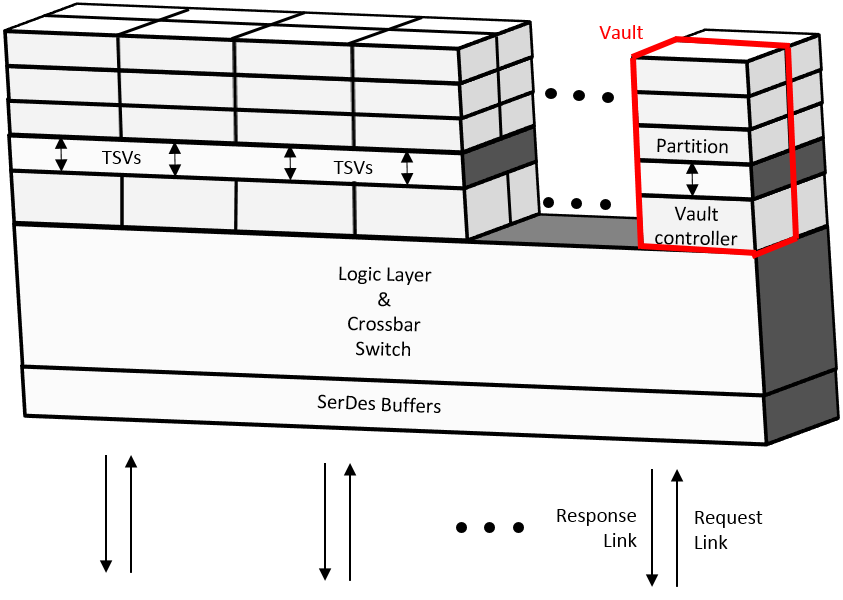
\includegraphics[width=0.75\linewidth]{figure/HMC_structures.png}
\caption{An example structure of a HMC chip }
\label{HMC-structure}
\end{figure}

Unlike DIMMs, which are either connected with pins and fastened with plastic clips or soldered at manufacturing, the HMC is designed to be included on the same substrate as the processor, known as 2.5D integration. This shortens the host-cube data paths, which requires less power to drive compared to the relatively long buses used with DDR memory. However, as with other stacked technologies, the issue with heat generation within the stack remains and might exceed the DRAM chips' maximum operating temperature of 85 °C \cite{7459470}. This could damage the chips and render the entire stack unusable. There are a number of proposed methods to solve this, either by static or dynamic memory mappings based on thermal properties. Hsieh et al shows what different mappings could look like, where memory is spread out in such a way that heat generation is as even as possible \cite{Hsieh:2013:TMM:2501626.2512457}. Additionally, since the logic (bottom) die is used for all accesses it will produce a lot of heat either way and therefore memory mapping should be done such that as little heat as possible is produced close to another hot spot.
\bigskip

Lastly, HMC support ECC in its specification, but the inclusion thereof is optional. Since one of the target markets for HMC is large-scale computing, ECC is an especially important feature. Since a host does not need any internal support for ECC either, it further reduces complexity and requirements on a connected host. HMC is not alone in supporting ECC as HBM also has this feature built-in.

\subsection{Interface}
Whereas DDR is designed so that the memory controller has full control over everything that happens, and the DRAM devices themselves are ''dumb'' devices, HMC moves the memory logic into the bottom cube layer and the vault controllers. In DDR communication, DRAM commands are sent directly from the CPU to the memory and get memory chunks in return. Here instead, the CPU communicates with the cube -- or a set of cubes, if that is the case -- over a general, packet-based protocol, which then at the receiving end (the logic layer) is converted into the device specific protocol. Unlike with DDR, this enables manufacturers to change the internal structure of the memory without having any compatibility issues with processors. Additionally, using an abstract interface enables less memory controller complexity inside the processor, which now only have to work with load/store operations instead of handling DRAM commands. Furthermore, having the memory controller stacked beneath the memory frees up valuable horizontal space on the CPU circuit, which can then instead be used for additional compute units or larger caches.  
\bigskip

The protocol used enables all cubes to address any vault, being local or remote. This in turn enables a host to be placed anywhere on the network and still be able to access the entire collective memory if needed. Using packet-based communication normally makes it possible to send parallel requests to multiple units, as is the case with HMC, and packets can contain a lot of information. The links between nodes contains several lanes, which by themselves are unidirectional but by having a lot of them the link can still be used with full-duplex. Before sending a minimal transmission unit, known as \emph{flits}, the packet must be serialised, which is handled by the SerDes interface. On the receiving end, the packets and de-serialised again and can be used for addressing DRAM again. This parallel protocol and multiple lanes per link allows for higher link bandwidth than the synchronous interface used by the normal JEDEC protocol. 
\bigskip

One of the main advantages of HMC is that it is made to be included on the same substrate as the processor, which shortens data paths dramatically compared to DIMMs attached to a PCB. This lowers the time it takes for data to travel to and from main memory,and also decrease the amount of energy needed to drive the buses. However, HMC also supports being soldered to the PCB, but that could potentially nullify this advantage in efficiency compared to DDRx memory. Thus, it is strongly recommended that cubes are on the same package \cite{hybrid2013hybrid}. By having memories at different logical and/or physical distances effectively makes the system a Non-Uniform Memory Access (NUMA) system. This is something that an OS needs to take into consideration when doing memory allocations as well as process scheduling. 
\bigskip

\subsection{Versions of HMC}
The first announcement of HMC was made public in 2011, and the 1.0 specification was published shortly thereafter. It was revised with version 1.1 later in 2012. It uses the architecture and interface described above, and links could utilise a maximum speed of 15GB/s. In 2014, the 2.0 specification was released, and specified a doubled maximum link speed to 30GB/s \cite{hybrid2014hybrid}. There are multiple versions of HMC being tested and produced currently, with everything from 2GB to 4GB cubes and with differing speeds. Future development consists of increasing the memory size of the HMC. While Intel initially announced Knight's Landing to use HMC 1.0 on board \cite{micron2014ikl}, there has as of yet not been released any commercial product using HMC.. 


%%%%%%%%%%%%%%%%%%%%%%%%%%%%%%  HBM  %%%%%%%%%%%%%%%%%%%%%%%%%%%%%%
\section{High Bandwidth Memory}
High Bandwidth Memory is, unlike HMC, a standard accepted by JEDEC \cite{standard2013high}. Although both HMC and HBM are different approaches to the same problem, their solutions differ somewhat. HBM is a stacked memory technology, and enables high bandwidth through parallelism and wide data interfaces while maintaining a nearly drop-in compatible interface with existing DDR memory controllers. This makes adoption easier compared to HMC, but there are still challenges among the benefits of performance.

\subsection{Architecture}
The stacked DRAM dies consisting of multiple banks are accessed through channels, where a maximum of eight channels per stack are split up between the layers. Banks are split into \emph{mats} of a matrix of DRAM cells, which in turn connects to a sense-amplifier or row-buffer. 32 such mats in one direction, a \emph{subarray}, are activated simultaneously when an access request arrives and each mat contributes 8 bits to the memory transaction of 32B in total -- an \emph{atom} \cite{7920815}. The banks communicate over an I/O buffer, which in turn connects to the external interface via on-die wires, TSVs between dies and then through wires in the base layer. Figure \ref{HBM-structure} shows an example, with 4 DRAM dies using 2 channels per die. These channels are fully independent, using separate clocks, timings and commands. Every channel uses a 128-bit wide interface, which with a maximum of eight channels gives a 1024-bit wide interface. Furthermore, each channel can transfer data at a rate of 1-2 Gb/s. Together with the wide data interface, HBM has the potential to deliver a bandwidth of 128 GB/s per stack. Each die can handle data capacities of up to 2 Gb, and with a maximum of 4 dies, HBM has a maximum size of 4 GB per stack \cite{7478812}.
\bigskip

Figure \ref{HBM-structure} also depicts that there is an optional logic die present. This die is optional, both in its existence and in its implementation and a vendor could develop it as a full memory controller. As the channels support Error-Correcting Code (ECC) memories, a controller could easily be made to support this as well. Even though the target market of HBM (graphics) might not be the most likely to need ECC, it is an available feature and could for, e.g., scientific applications be a welcome addition. Having a logic die present can save energy by being the sole handler of, e.g., refreshing DRAM banks. This would decrease the amount of data needed to be sent over the substrate interconnect. However, this is not the largest contributing factor to a device's power usage. 
\bigskip

In an HBM stack, the biggest addition to the total power consumption is row activation, where data is being read from the cells. Next most power goes to moving data inside a chip, between different layers and inside the interposer -- in descending order. The highly parallel interaction with the memory banks consumes a lot of power and makes overall power utilisation high. Although HBM consumes a lot of power, it does so with extreme bandwidth and therein lies the trade-off. Compared to DDR4 memories, HBM uses about 5 times less energy per transferred bit. As such, the efficiency of HBM is tremendous, but any system using it must have a large power and thermal budget to be able to accommodate it in a system design.
\bigskip

HBM was co-developed by AMD, whose main use for it was going to be graphics processing units (GPUs). One example in the HBM architecture that shows that this is primarily is aimed for graphics applications today is that the atom size is 32B. This size could be increased to gain pure bandwidth, which for many general applications could be beneficial. Graphics applications use this specific size for optimisations, e.g. because GPUs compress surface tiles to 32B entities, and using a larger size atom, e.g. of 128B, would create an overfetch of data. This would decrease overall performance by 17\% \cite{O'Connor:2017:FDE:3123939.3124545}. However, HBM is more and more being viewed as a solution to memory bound AI applications \cite{sperling_2019}.

\begin{figure}[!ht]
\centering
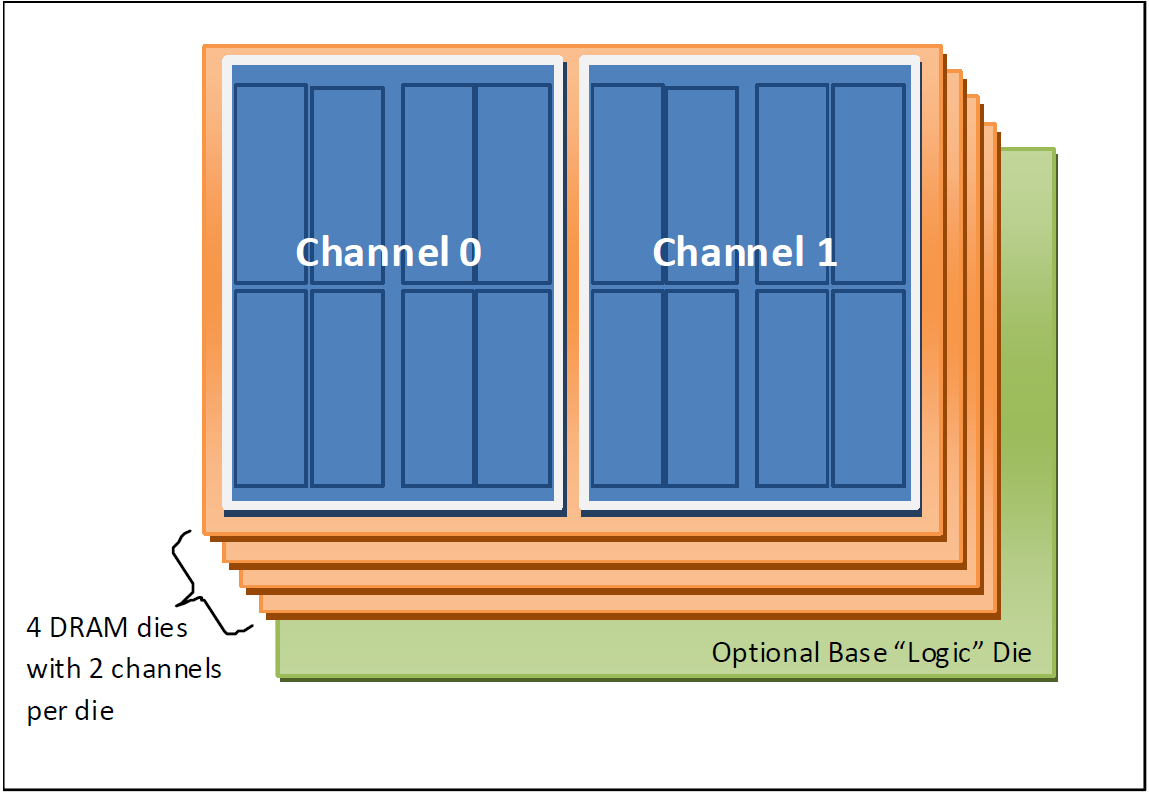
\includegraphics[width=0.75\linewidth]{figure/HBM_structure.PNG}
\caption{The structure of a HBM chip. Image courtesy of JEDEC 2013 }
\label{HBM-structure}
\end{figure}

\subsection{Interface}
The optional logic die in the specification allows developers to chose to integrate HBM with existing memory designs, utilising an already present memory controller, or they can choose to create a new one. However, since the interface is different from that of DRAM, an existing memory controller would still need to be updated according to HBM specification. Even so, this provides a flexible way to more easily allow quick adoption of the memory type. TODO: Source and/or example would be great here.
\bigskip

An HBM stack communicates with the memory controller, i.e. the CPU, through the interposer using 1024 I/Os. Having this many I/Os causes great power usage if all memory logic were to be placed on the CPU side, but by instead having a logic die in the base of the HBM stack this consumption can be decreased significantly. Like HMC, HBM is based on 2.5D silicon interposer integration. In contrast to HMC, however, HBM does not support being built on the PCB. Because of its very wide interface, it would require too much energy to power such communication buses. Thus HBM is required to be built close to the processor, on the same substrate.

\subsection{Versions of HBM}
While the initial version of HBM was released in 2013 \cite{standard2013high}, HBM2 was released in 2015 \cite{standard2015high} and provided some anticipated improvements. One of the most important was the increased capacity by allowing up 8-Hi stacks while maintaining the same 1024 bit wide interface. At the same time, the maximum bandwidth was increased to 256 GB/s by utilising overlapping accesses to bank groups over multiple cycles \cite{O'Connor:2017:FDE:3123939.3124545}. This required an increase in frequency up to 1.2 GHz as well. Both HBM and HBM2 has been used in commercial GPUs and acceleration cards but their use is still limited. This is most likely due to their high cost as compared to (G)DDR memories in combination with the issues arising from limited power budgets and thermal dissipation.
\bigskip

In 2018 HBM2E specification was released, further increasing maximum bandwidth to 306 Gbit/s and density to 16 Gb per die \cite{standard2018highe}. In addition, 12-Hi stacks are now supported, allowing up to 24 GB per stack. Samsung managed to manufacture such a stack while maintaining the same stack height, which is important for integration in existing systems \cite{liu_2019}. There are plans for both HBM3, HBM3+ and HBM4, all of which are aiming to further increase bandwidth, capacity and lower costs. In addition, there has been talks of creating a special specification for a lower power version of HBM2 as well, using a 64 bit wide interface per channel. This could dramatically reduce power at the expense of some of the bandwidth, but more suited for mobile applications. This has however not been released officially. 


%%%%%%%%%%%%%%%%%%%%%%%%%%%%%%  WIO  %%%%%%%%%%%%%%%%%%%%%%%%%%%%%%
\section{Wide-IO}
While HBM and HMC aim at delivering as much performance as possible, Wide-IO (WIO) targets smaller, mobile devices with limited available power and small thermal envelope. Therefore, WIO targets high energy efficiency and low power consumption, rather than highest possible performance. Additionally, unlike HMC and HBM, WIO is designed for 3D chip-on-chip integration on System on Chips (SoCs). This enables even shorter, lower capacitance data paths compared to 2.5D as used by HMC and HBM. Like HBM, Wide-IO is a JEDEC standard, and was first accepted in 2011 \cite{standard2011wide}. 

\subsection{Architecture}
Wide-IO is based on stacked Single Data Rate (SDR) memory dies and uses a signalling system quite similar to that of standard DDR memories. Communication from the single memory controller is handled through four 128-bit wide physical channels. Additionally, there are four logical channels, which are controlled separately by the physical channels. The physical channels have access to all the data, control and clock logic to independently manage the logical channels, meaning that each logical channels can have their own memory pages open while also having individual clock and power states. A Wide-IO stack can consist of between one to four DRAM dies and each part of the slice belonging to a physical channel is denoted as a rank. Stacks can utilise capacities between 128MB up to 4GB. 
\bigskip

While being mostly based on and often compared to (LP)DDR memory, WIO can have internal structures that alters its performance but not its compliance against the standard. This is shown in \cite{6487803}, where Takaya et al managed to achieve 100 GB/s by using a larger number of TSVs and a three level chip stack with an active interposer inside. In addition, the placement of interconnects and the path taken to the host/logic chip also matters; placing the chips either "face-to-face" or "face-to-back" can have an impact on performance and stacking density \cite{6248798}.

TODO: Find and insert a small graphic of WIO here!

\subsection{Interface}
The memory controller is very similar to a standard SDRAM controller. Since commands are similar to those in DDR, it makes the controllers resembling one another. The biggest difference being that that in the target market (mobile) there are more often than not only one or two memory channels available, while there in Wide-IO are four. Each channel is 128 bits wide, which provides the memory an aggregated 512 bits interface. WIO has a bandwidth of 17 GB/s -- 4,26 GB/s per channel. TODO: something more?!
\bigskip

Wide-IO is, unlike both HMC and HBM, primarily aimed at being 3D, chip-on-chip integrated. While the standard supports 2.5D integration, it is not recommended for optimal performance. However, as the latter integration technique gives rise to fewer problems, this will most likely be the initial approach. While there certainly are challenges in manufacturing stacked memory it is far from impossible to create working 3D chips with reasonable yields; Kim et al. managed to create a 4-Hi WIO stack with an expected yield of 76\% \cite{kim20121}. TODO: Reference back to section talking about comparison between 2.5D and 3D integration performance and cost.

\subsection{Versions of WIO}
The first version was accepted by JEDEC in 2011, and a new specification for Wide-IO2 (WIO2) was accepted and released in 2014. WIO2 uses 64-bit wide channels instead of 128-bit, but the maximum amount of channels has increased to eight. It is still allowed to just use four channels, but there are no longer any logical channels available to further increase parallelism inside. Since there no longer are channels which share control logic -- which physical and logical channels did previously -- each channel is now fully independent. The density of one chip has stayed the same (32Gb), but accepted densities now start from 4Gb instead of 1Gb. The main improvement lies in the maximum bandwidth stacks are capable of -- it has increased from 17GB/s to 68GB/s. Additionally, WIO2 no longer use SDR, but instead utilise DDR signalling. \cite{standard2014wide}.

\section{A Comparison of Emerging Technologies}
While all of these emerging memory technologies promises boosts in performance as well as efficiency compared to today's memory devices, there are still ongoing research regarding additional memory architectures. One such is Fine-Grained DRAM (FGDRAM) which O'Connor et al claims provides four times the bandwidth at 50\% of the power per access compared to HBM2 \cite{O'Connor:2017:FDE:3123939.3124545}. Another proposal comes from Chatterjee et al whose DRAM architecture and new memory controller manages to use 35\% less energy and perform 13\% better for GPU applications compared to an HBM baseline \cite{7920815}. As such, stacked memory is not the one way forward either, but it still presents great potential. Even though other designs might perform better, they may also still use the same amount of die area as today's solutions; area which could perhaps otherwise be spent on compute units which could even better utilise the increased available bandwidth. The main conclusion to make is that simply continuing to rely on the current evolutionary improvements of DDR will likely not result in neither the most efficient nor the most performant solution.
\bigskip

The Non-Volatile memory technologies mentioned in the beginning of the \nameref{background} are one way to approach the stagnant memory performance seen today, but their maturity are still a few years off in the future. Likewise, there are maturity issues with these stacked technologies; the cost of designing and manufacturing systems with an interposer as well as making a trade-off between performance and heat in a system are large investments to overcome. This is likely the reason why WIO, in either of its versions, has not taken off very well, as 3D integration still poses many problems for large scale manufacturing. 2.5D integration is currently the more viable design, and here HBM and HMC outperform WIO. However, while HBM and HMC are using a logic die as the bottom, interface die, WIO does not. For the two former technologies it makes sense to have these present as it will lower the power consumption since it decreases the travel for every memory request. For WIO however, the memory is placed so close to the CPU (on top of) that an additional logic layer simply would increase complexity and use unnecessary resources. HBM has already been shipped with multiple devices and HMC has been announced to ship with some Intel devices. Intel has, however, announced an architecture named Foveros which stacks memories and logic together in several layers (four low power Atom cores together with one large Sunny Cove core), and as such there might be more 3D integrated, unannounced designs on the horizon. TODO: add source for Foveros.
\bigskip

WIO and HBM build upon existing interfaces and signalling schemes, which already have gotten a lot of improvements over the years, as opposed to HMC which relies on a packet-based network interface. This means both that there would be many new things to take into consideration while designing systems with HMC memory, but also that operating systems need to be adopted as well. Since this normally is not something done by memory chip manufacturers this would add an extra layer of complexity to get HMC to market. Since developing electronic devices is costly time to market is important, and here HBM and WIO has the advantage. However, HMC has the benefit of being targeted more for general computation rather than mainly graphics applications; HBM is wide and slow, whereas HMC is both fast and wide. If you have applications that don't need much memory at a time but need it fast, HBM is arguably going to perform worse than HMC. This could be solved to some extent by using either memory in combination with other memory types, and create a hybrid memory. In addition, the target market for the system also needs to be considered -- WIO would be a worse choice in a data centre than HMC, while HMC in turn would consume too much energy to act as the sole primary memory in a mobile unit.
\bigskip

Another interesting aspect of HMC is its added network functionality, which opens up the possibility to use multiple cubes and hosts on the same network. This could potentially scale well for servers utilising multiple processors and are to some extent already working on the same data. The communication between remote memory cubes and hosts only consists of a protocol as far as the specification goes, and it would still need a physical interface to travel between network nodes, e.g. Ethernet, or CXI or CXL if nodes have a connection over PCI Express. In addition, the networking capabilities of HMC allows a host to be connected anywhere in a network which perhaps can create further opportunities for scalable computer systems which yet remain unexplored. This, however, raises the question how multiple cubes perform together and how having a multi-hop main memory affects performance. Servers and data centres are often meant to be fast, and if having several HMCs in the same network affects performance then one of their main differentiators only add overhead. Having multiple hops increases latency, and it would be interesting to study how performance is affected by introducing several hops in page lookups.
\bigskip
